%%%%%%%% ICML 2027 SUBMISSION %%%%%%%%%%%%%%%%%%%%%%%%%%%%%%%%%%%%%%%%%%%%%%%%%%%%

% The paper: MicroInfer and semantic-aware adaptive KV cache precision, in the
% ICML 2027 format (icml2027.sty and icml2027.bst, from the official style
% package at icml.cc; example_paper.pdf is its instructions). Every figure
% quoted must come from experiments/logs/benchmark.jsonl; entries are cited by
% their sha256 prefix in the ADRs. The main body must stay within eight pages;
% references, the statements and the appendix do not count. The folder is
% self-contained, so that it compiles as uploaded.

\documentclass{article}

\usepackage{microtype}
\usepackage{graphicx}
\usepackage{booktabs}

% hyperref before icml2027, as in the official example. If a build breaks on a
% link that spans a page, drop this line and pass [nohyperref] to icml2027.
% The style's \printAffiliationsAndNotice sets its footnote with \thefootnote
% empty, for which a footnote link would have an empty anchor; the paper has
% no other footnote, so footnotes are not linked.
\usepackage[hyperfootnotes=false]{hyperref}

% Submission: anonymised. Use [preprint] for arXiv, or [accepted] once
% accepted; either prints the authors and the acknowledgements.
\usepackage{icml2027}

\usepackage{amsmath}
\usepackage{amssymb}
\usepackage{nicefrac}
\usepackage{adjustbox}
\usepackage{tikz}
\usetikzlibrary{arrows.meta}

% A table no wider than its column is left alone; a wider one is shrunk to fit,
% by adjustbox's max width.

\icmltitlerunning{Reallocating KV Cache Precision at Runtime under Video Memory
Contention}

\begin{document}

\twocolumn[
  \icmltitle{Keeping Local LLM Inference Alive under Video Memory Contention
    \texorpdfstring{\\}{ }by Reallocating KV Cache Precision at Runtime}

  % Printed only with [accepted] or [preprint]; the submission shows
  % "Anonymous Authors" whatever is written here.
  \begin{icmlauthorlist}
    \icmlauthor{Firstname Lastname}{hust}
  \end{icmlauthorlist}

  \icmlaffiliation{hust}{School of Information and Communications Technology,
    Hanoi University of Science and Technology, Hanoi, Vietnam}

  \icmlcorrespondingauthor{Firstname Lastname}{email@domain}

  \icmlkeywords{LLM inference, KV cache quantization, mixed precision, GPU
    memory contention, consumer hardware}

  \vskip 0.3in
]

% Required, with empty braces when there is no special notice.
\printAffiliationsAndNotice{}

\begin{abstract}
On a consumer GPU, video memory is shared without isolation with a browser, a
video player and an editor, so another process taking memory can end a local
language model session with an out-of-memory error and lose its context. We
present \textit{MicroInfer}, an inference engine built from scratch in which
every page of the key-value cache carries its own precision tier among FP16,
INT8, INT4 and INT2, and a control loop, a pressure monitor polling the driver
with thresholds derived from measured contention, an importance scorer inside
the attention kernel and a marginal-cost planner, downgrades the pages whose
loss costs least per byte, returns the freed memory to the driver, and restores
the pages exactly from a host-memory copy once pressure passes. On a 6\,GiB
laptop GPU, everyday applications take hundreds of MiB and mostly keep them,
and the monitor detects every catchable episode within 236\,ms with no false
positive. With Qwen2.5-1.5B at 32K positions, the adaptive engine survives a
contention that runs the static engine out of memory, returning 746\,MiB that
the driver sees returned, and across four scenarios of three runs each it
survived every run the static engine failed but one that exceeded the device;
llama.cpp, which reserves its cache at load, survives as well, its FP16 cache
refusing the other process up to 364\,MiB.
At equal reclaimed bytes and 80\% of them reclaimed, attention-guided
allocation keeps the next-token distribution 3.6 times closer to full precision
than uniform allocation, where a page's score ranks its downgrade's damage
($\rho = 0.36$), but answers no more of an easy needle set, 48 of 50 against
49, where it does not ($\rho = 0.03$). On five RULER tasks below their ceiling
it answers more at 80\%, 123 of 250 against 100 at 8K and 100 against 52 at
32K ($p \le 0.0032$), mostly on variable tracking, and fewer at 70\% where
needle-shaped fillers hide the needle; on a second family, Llama-3.2-1B, it
answers 134 against 58 at 8K and 80\%. The planner takes any score: ZipCache's,
probed over the prompt, answers as many at 8K and 80\% (132, $p = 0.20$) and
more at 70\% (245 of 250 against 206), ahead of uniform allocation at both.
Downgrading keeps 48 needles where evicting the same bytes keeps 16.
\end{abstract}

% =====================================================================
\section{Introduction}
\label{sec:introduction}

Large language models are increasingly run on personal hardware. Openly
released models of one to a few billion parameters \citep{qwen2024report},
together with tools such as Ollama \citep{ollama} and llama.cpp
\citep{llamacpp}, make it ordinary to hold a conversation with a model on a
laptop, for privacy, offline use, and the absence of a per-token bill. Wherever
a model runs, its inference is bound by memory: generating a token reads every
weight and every cached key and value, and in datacenter serving the memory the
key-value cache takes is what limits how many requests are served at once
\citep{kwon2023pagedattention}. On a laptop the limit is tighter, a few GiB of
video memory for weights, cache and working space together.

On a consumer graphics processor that memory is not even fixed. Unlike a
datacenter accelerator partitioned by MIG or MPS, a consumer GPU offers no
memory isolation between the processes that share it: video memory goes to
whoever asks first, and no process is told when another takes more. A session
that fits comfortably can then fail outright when a browser tab starts playing
video. The failure is not degradation but termination: the session ends and its
cached context is lost. On the 6\,GiB laptop GPU used here, everyday
applications take hundreds of MiB and mostly keep them, which brings a long
session to within a few hundred MiB of that failure (Section~\ref{sec:rq1}).

What makes the problem tractable is that a model's footprint is not
monolithic. Its weights are fixed for a session, but its key-value cache grows
with every token and can be held at varying precision; at a long context,
compressing it frees as much memory as an everyday application takes. We ask
whether that trade can be made \textit{during} a session, in response to
pressure the engine did not cause, and whether the loss can be concentrated on
the cached positions the model attends to least.

Existing work holds parts of the answer (Section~\ref{sec:related}). Adaptive
serving systems change memory allocation at runtime, but for pressure that
comes from the requests they admit. Consumer engines run in the right place,
but fix capacity when the model loads. Uniform cache quantisation settles how
far a cache can be compressed, and mixed-precision quantisation shows that
precision is better spent unevenly, guided by attention or sensitivity; both
fix their budget before the session. Attention-guided eviction has the right
signal but discards irreversibly. No system reallocates cache precision at
runtime, non-uniformly, in response to memory taken by processes it cannot see,
and restores it afterwards.

This paper asks three questions, each answered by a component of the system.
\textbf{RQ1:} how volatile is free video memory on a consumer laptop under
everyday use? We record it at 50\,Hz while a script plays everyday
applications, and analyse every spike by a rule fixed before recording.
\textbf{RQ2:} can a runtime that consults no scheduler detect pressure, and
survive it? A monitor polls the driver with thresholds set by a rule from RQ1's
spikes, and a controller downgrades cache pages to meet a byte target; we score
the monitor against an independent ground truth and run a session through
contention that ends the static engine. \textbf{RQ3:} does allocating
precision by attention preserve task quality better than allocating it
uniformly, at equal compression? Four score sources, ours, a published rule's
and two controls, plug into the same planner, so that they reclaim the same bytes
and differ only in which pages they degrade.

Our contributions are:
\begin{itemize}
\item \textbf{A characterisation of video memory contention on a consumer
laptop}, attributed to the processes that cause it: spikes are large (P90
506\,MiB), rise over seconds (median 1.09\,s) and mostly persist (45 of 48).
\item \textbf{A scheduler-agnostic pressure monitor} whose thresholds follow
from that measurement by a fixed rule, and which detected all 84 catchable RED
episodes within 236\,ms with no false positive.
\item \textbf{A runtime precision policy and the engine that runs it}: a paged
cache whose pages change tier between decoding steps, every move quantising
from an FP16 shadow so that upgrades restore exactly, freed memory returned to
the driver, and a marginal-cost planner that takes its page scores from any
source. It survives, at 32K positions, a contention that ends the static
engine.
\item \textbf{An evaluation design that isolates allocation from compression},
holding the reclaimed bytes equal between score sources and eviction. At 80\%
of the bytes reclaimed, attention-guided allocation kept the output distribution
closer to full precision than uniform (mean KL 0.028 against 0.101) and answered
more of RULER's tasks below their ceiling (100 of 250 against 52 at 32K), though
no more of an easy needle set, and downgrading kept three times the answers of
evicting the same bytes. Our score is not the best of them: ZipCache's, on the
same planner, answered more of RULER at 70\% and no fewer at 80\%.
\end{itemize}

% =====================================================================
\section{Background and Related Work}
\label{sec:related}

\paragraph{The key-value cache.} Decoding attends over all previous positions
\citep{vaswani2017attention}, so their keys and values are cached. The cache
takes $2 \cdot L \cdot h_{kv} \cdot d_h \cdot n \cdot s$ bytes for $L$ layers,
$h_{kv}$ key-value heads of dimension $d_h$, $n$ positions and $s$ bytes per
element. Of these, only $n$ and $s$ change during a session, and $n$ is the
user's: bytes per element is the one term an engine can renegotiate. On
Qwen2.5-1.5B a position takes 28\,KiB at FP16, so 32K positions take 896\,MiB;
at a short context, compressing the whole cache frees less than a browser tab
takes, which fixes our experimental configuration at a long one.

\paragraph{Video memory on consumer GPUs.} Free memory is observable only by
polling the driver \citep{nvml}, and only memory returned to the driver is
visible there: a caching allocator that keeps freed memory makes it look like
contention. The CUDA virtual memory management interface \citep{cudavmm}
reserves address ranges independently of physical memory, so a cache can map
memory granule by granule and give it back.

The related work falls into five families, which we take from the furthest from
this work to the closest.

\paragraph{Adaptive serving.} PagedAttention \citep{kwon2023pagedattention}
manages the cache in blocks inside a reservation taken at start-up. FineServe
\citep{fineserve} serves models of heterogeneous precision, MorphServe
\citep{morphserve} swaps in quantised layers and resizes the cache with the
workload, Oneiros \citep{mirage} remaps parameter memory to hold more cache,
and eLLM \citep{ellm} manages memory elastically. They show runtime adaptation
is worthwhile, but assume a dedicated accelerator, a scheduler that sees the
pressure coming, and many requests to trade between; and memory kept in a
private reservation is never returned to the driver.

\paragraph{Consumer and edge inference.} llama.cpp \citep{llamacpp} and Ollama
\citep{ollama} bring quantised models to personal machines, PowerInfer
\citep{song2024powerinfer} splits work between GPU and CPU by neuron activity,
and FlexGen \citep{sheng2023flexgen} offloads to host memory and disk. They
treat capacity as fixed when the model loads; Section~\ref{sec:survival}
measures what that means for llama.cpp under contention.

\paragraph{Uniform cache quantisation.} KVQuant \citep{hooper2024kvquant} and
KIVI \citep{liu2024kivi} show that the cache tolerates aggressive quantisation;
KIVI quantises keys per channel and values per token and reaches two bits. We
adopt KIVI's quantiser. Its precision is chosen once, before the session, and
identically for every position.

\paragraph{Attention-guided eviction.} H2O \citep{zhang2023h2o} keeps the
tokens that accumulate attention, StreamingLLM \citep{xiao2024streamingllm}
keeps the initial ``attention sink'' with a recent window, and Ada-KV
\citep{feng2024adakv} spreads the budget across heads. We borrow the signal;
eviction itself is irreversible and its budget fixed.

\paragraph{Mixed-precision cache quantisation.} The closest family varies
precision across the cache: KVTuner \citep{kvtuner} by layer from offline
sensitivity, MiKV \citep{yang2024mikv} by keeping tokens an eviction policy
would drop at low precision, ZipCache \citep{he2024zipcache} by salient tokens
found from normalised attention, and Cocktail \citep{tao2025cocktail} by chunk
from similarity to the query. They distribute a budget fixed in advance and
observe nothing of the memory the device has left, and none raises precision
again.

% =====================================================================
\section{Design}
\label{sec:design}

\subsection{Overview}
\label{sec:overview}

\textit{MicroInfer} has two layers (Figure~\ref{fig:overview}). The
\textbf{engine} runs the model over CUDA kernels written for this work and
holds the cache on \textit{pages}, the keys and values of $P = 32$ consecutive
positions of one layer, each at a \textit{tier}: FP16, INT8, INT4 or INT2. The
\textbf{control loop} decides which page is held at which tier: a pressure
monitor, an importance scorer, a precision controller, and the cache manager
that applies its plans. Plans are applied between decoding steps, never inside
a kernel launch, so no kernel sees the cache half converted.

\begin{figure}[t]
\centering
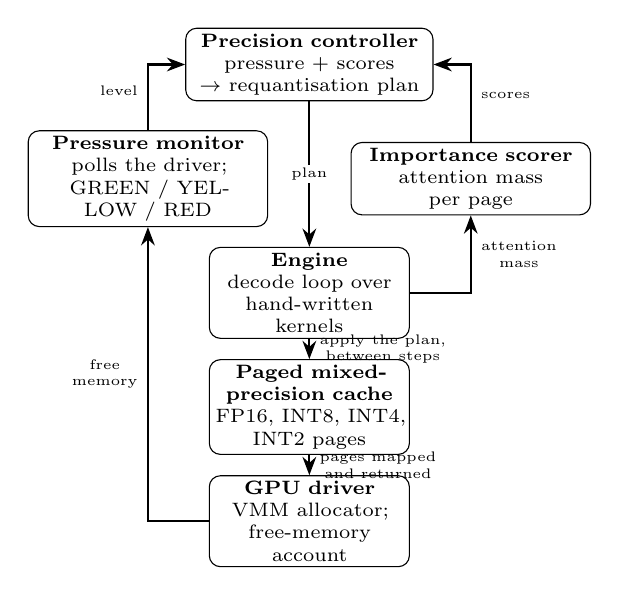
\begin{tikzpicture}[
  box/.style={draw, rounded corners, align=center, minimum height=0.85cm,
              inner sep=2pt, font=\scriptsize},
  arrow/.style={-{Stealth}, thick},
  note/.style={font=\tiny, align=center}]
  \node[box, text width=3.0cm] (controller) at (0, 3.35)
    {\textbf{Precision controller}\\pressure + scores\\$\rightarrow$ requantisation plan};
  \node[box, text width=2.9cm] (monitor) at (-2.05, 1.9)
    {\textbf{Pressure monitor}\\polls the driver;\\GREEN / YELLOW / RED};
  \node[box, text width=2.9cm] (scorer) at (2.05, 1.9)
    {\textbf{Importance scorer}\\attention mass\\per page};
  \node[box, text width=2.4cm] (engine) at (0, 0.45)
    {\textbf{Engine}\\decode loop over\\hand-written kernels};
  \node[box, text width=2.4cm] (cache) at (0, -1.0)
    {\textbf{Paged mixed-precision cache}\\FP16, INT8, INT4,\\INT2 pages};
  \node[box, text width=2.4cm] (driver) at (0, -2.45)
    {\textbf{GPU driver}\\VMM allocator;\\free-memory account};
  \draw[arrow] (driver.west) -| node[note, pos=0.75, left] {free\\memory} (monitor.south);
  \draw[arrow] (monitor.north) |- node[note, pos=0.3, left] {level} (controller.west);
  \draw[arrow] (engine.east) -| node[note, pos=0.75, right] {attention\\mass} (scorer.south);
  \draw[arrow] (scorer.north) |- node[note, pos=0.3, right] {scores} (controller.east);
  \draw[arrow] (controller.south) -- node[note, fill=white, inner sep=1pt] {plan} (engine.north);
  \draw[arrow] (engine.south) -- node[note, right] {apply the plan,\\between steps} (cache.north);
  \draw[arrow] (cache.south) -- node[note, right] {pages mapped\\and returned} (driver.north);
\end{tikzpicture}
\caption{\textit{MicroInfer}: the engine, and the control loop that decides the
precision tier of each page of its key-value cache. Freed memory returns to the
driver, where the monitor and other processes see it.}
\label{fig:overview}
\end{figure}

\subsection{The Pressure Monitor}
\label{sec:monitor}

A background thread polls the driver's free memory, the \textit{headroom},
every 50\,ms on absolute deadlines. Headroom below $T_\mathrm{low}$ is RED,
below $T_\mathrm{high}$ YELLOW, else GREEN; thresholds are absolute, since
contention is. A new level is reported once $K$ consecutive polls agree, so a
drop shorter than $K$ polls is never reported and a clean change is reported
within $K+1$. Each transition is queued as an event, with the memory held by
the engine and by every other process.

The thresholds follow from RQ1 by a fixed rule, not by tuning. RED is headroom
below a spike at the P90 amplitude, rounded up to 64\,MiB; $K$ is the largest
number of polls whose detection time, $(K+1) \times 50$\,ms, does not exceed the
P10 rise time; YELLOW adds what a fast spike takes while it is detected and a
plan applied. RQ1's spikes give RED below 512\,MiB, $K = 3$ and YELLOW below
1024\,MiB.

\subsection{The Mixed-Tier Paged Cache}
\label{sec:cache}

Quantised tiers follow KIVI \citep{liu2024kivi}: keys asymmetric with a scale
and zero-point per (head, channel) across the page, values per (head,
position). One layout serves every tier; its 1280 bytes of metadata per page
on Qwen2.5-1.5B make INT8, INT4 and INT2 cost 8.63, 4.63 and 2.63 effective
bits per element, and every compression ratio here counts it. A page being
filled stays at FP16, since a key channel's scale spans the whole page.

Each tier has its own virtual address range, reserved through the VMM interface
for the whole context window. Physical memory is mapped a 2\,MiB granule at a
time as pages arrive; a tier's live pages occupy its lowest slots, freeing a
page moves the tier's last page into its slot, and an empty granule is returned
to the driver. One attention kernel reads every page at the tier the page table
records for it, dequantising as it loads, in a single pass; query tiles are
aligned to pages, so a tile reads one tier.

\subsection{Runtime Requantisation}
\label{sec:requantisation}

A downgrade allocates the page at the target tier while the old page is still
read, quantises it, points the page table at it, and frees the old page; if
the allocation fails, nothing has changed. Before a page's first downgrade its
FP16 bytes are copied to pinned host memory, its \textit{shadow}, and every
move quantises from FP16, never from the current codes. A page at tier $T$ is
therefore always exactly the quantisation of its rows at $T$: each tier has one
error, and errors do not compound along a page's path. An upgrade copies or
quantises from the shadow; to FP16 it restores the page bit for bit. Decoding
the codes back up was rejected, since it would give FP16's size at the lower
tier's error. A move of one page of one layer takes 8 to 39\,$\mu$s at the
median on Qwen2.5-1.5B (Appendix~\ref{app:moves}), and the shadows of a whole
32K cache take about 0.9\,GiB of host memory. The tier a cache is held at
changes its decoding speed: at 32K positions, against FP16 at the same code, a
cache at INT8 decoded 31\% faster, one at INT4 24\% slower and one at INT2 48\%
slower, one run each (Appendix~\ref{app:moves}); two FP16 runs at different
commits differed by 16\%.

\subsection{The Importance Scorer}
\label{sec:scorer}

The attention kernel computes the softmax online, one page per tile. On
request each tile writes its partial $\sum \exp(s - m)$ with its maximum $m$,
and once the softmax's final maximum and sum are known these are normalised
into each page's share of the attention mass, with no second pass over the
cache. Averaged over a layer's query heads, the mass $\bar a_{\ell,i}$ of page
$i$ in layer $\ell$ is folded on the device into
$\mathrm{score}_{\ell,i} \leftarrow \alpha\,\bar a_{\ell,i} + (1-\alpha)\,
\mathrm{score}_{\ell,i}$ with $\alpha = 0.2$, a page's first observation
seeding its score. Folding every step cost Qwen2.5-0.5B 0.71\% of decode
throughput, outside noise; every fourth step is within noise on both models and
is the default. Attention sinks get no special protection: unaided, the scorer
rates the first page highest when averaged over layers.

\subsection{The Precision Controller}
\label{sec:controller}

The controller, pure logic with no device code, turns the level, the headroom,
the scores and the tiers into a plan. It reclaims what brings headroom back
above YELLOW with a 64\,MiB margin, $T_\mathrm{high} + 64\,\mathrm{MiB} -
\text{headroom}$, rather than a fixed fraction of the cache. It meets this
target greedily, repeatedly taking the cheapest next move of one page one tier
down by marginal cost
\begin{equation}
  c_{\ell,i}(t \to t') = \mathrm{score}_{\ell,i}\,
    \frac{e(t') - e(t)}{b(t) - b(t')},
  \label{eq:marginal}
\end{equation}
where $e$ is a tier's relative mean squared error from offline round trips and
$b$ its bytes per page. Equal scores give breadth first, since each tier down
costs more per byte than the last; a page the model hardly attends to goes deep
first. The open pages and the last 128 positions are never downgraded.
Upgrades come at GREEN only, largest gain first, at least 5\,s after the later
of the last downgrade and the end of pressure, and never below $T_\mathrm{high}
+ 512$\,MiB of headroom. Any \textit{score source} plugs into the same
planner and meets the same byte target to within one page's move. At runtime it
is the scorer's (\textit{semantic}), equal scores spread evenly across positions
(\textit{uniform}, the baseline), or seeded random scores; RQ3 adds ZipCache's.

\paragraph{The engine's reaction.} On YELLOW the engine applies the plan a
batch per step within 20\,ms; on RED, all at once; while the level persists it
plans again as the cache seals pages. If an allocation fails outright, an
emergency plan for no headroom is applied and the step retried once; failing
that, the generation ends gracefully with the tokens it produced. Because events
are drained only between steps, and a 512-position prefill chunk at 16K--24K
positions takes 11--16\,s, prefill chunks are sized under pressure from a model
of a step's cost, a fixed part plus a part per position, so that a step takes
about 0.8\,s, or about twice its fixed part where the fixed part alone exceeds
that. At GREEN chunks stay at 512 positions.

% =====================================================================
\section{Implementation}
\label{sec:implementation}

\textit{MicroInfer} is a Python orchestrator over CUDA kernels written for
this work: embedding, RMSNorm, rotary embeddings, SwiGLU, attention over
contiguous, paged and quantised pages, the paged cache and its VMM allocator,
quantisation at every tier, and greedy sampling. No other
inference engine is part of it; llama.cpp is run only as a baseline beside it.
The one exception to hand-written kernels is the dense projections, which call
cuBLAS \citep{cublas} with fp32 accumulation; hand-written GEMMs ran 8--28 times slower at 512 rows,
and would have confounded every latency we report with the cost of a slow
matrix multiplication (Appendix~\ref{app:boundary}). No deep learning
framework runs beside the engine, whose caching allocator would hide freed
memory from the driver. Every figure below is drawn from a hash-chained
benchmark log whose entries name the code that produced them.

% =====================================================================
\section{Evaluation}
\label{sec:evaluation}

All measurements are on one laptop with an NVIDIA RTX 4050 Laptop GPU (6\,GiB,
6141\,MiB reported by driver 580.178.04), an Intel Core i7-13650HX and
23.2\,GiB of host memory, under Linux 6.14 with CUDA 12.9 and a GNOME desktop
whose processes share the GPU throughout. The experimental configuration is
Qwen2.5-1.5B at 32K positions with its cache at FP16, which leaves about
1.2\,GB of headroom: the range in which realistic contention decides whether a
session survives. Llama-3.2-1B-Instruct \citep{llama3herd}, with eight key-value
heads against two, runs a subset (Appendix~\ref{app:llama}).

\subsection{RQ1: Contention on a Consumer Laptop}
\label{sec:rq1}

A script played everyday actions, labelling each in the trace: a browser with
1, 5 and 10 tabs, YouTube at 1080p and 2160p, a WebGL page, a 2160p video in
VLC, and VS Code. A recorder sampled free memory at 50\,Hz and each process's
memory at 5\,Hz. The scenario was recorded five times with the engine holding
32K positions and once without it, 2.2 hours in all, and analysed by a spike
definition fixed beforehand (Appendix~\ref{app:spikes}): free memory at least
64\,MiB below a rolling 5\,s median for at least 100\,ms.

\begin{table}[t]
\caption{Spikes at the 64\,MiB threshold in six recordings, by the action in
progress, with their median and largest amplitude. Contention is large, and a
video player takes the most.}
\label{tab:rq1}
\centering
\small
\begin{adjustbox}{max width=\columnwidth}
\begin{tabular}{lrrr}
\toprule
Action & Spikes & Median (MiB) & Largest (MiB) \\
\midrule
Browser, 10 tabs & 7 & 220 & 284 \\
Browser, 1 tab & 6 & 150 & 167 \\
VLC, 2160p video & 6 & 526 & 567 \\
YouTube, 1080p / 2160p & 5 / 5 & 101 / 181 & 292 / 196 \\
VS Code & 5 & 91 & 94 \\
Engine prefill & 5 & 182 & 182 \\
WebGL page & 4 & 100 & 138 \\
Other & 5 & 85--103 & 103 \\
\bottomrule
\end{tabular}
\end{adjustbox}
\end{table}

The six recordings hold 48 spikes (98 at 32\,MiB, 28 at 128\,MiB;
Table~\ref{tab:rq1}). \textbf{Contention mostly stays:} 45 of the 48 are lasting
drops, an application keeping its memory until it closed, so reclaiming memory
once is not enough. \textbf{It is large:} a median of 154\,MiB, a P90 of
506\,MiB, and at most 567\,MiB. \textbf{It rises over seconds:} a median of
1.09\,s from 10\% to 90\% of the amplitude, and a P10 of 242\,ms. Attribution
named a process for 44 spikes, mostly the browser's GPU process
(Figure~\ref{fig:spikes}). Beside the
engine at 32K the lowest headroom was 377\,MiB: contention brings a long
session within a few hundred MiB of failure.

\subsection{RQ2: Detecting Pressure}
\label{sec:detection}

The monitor was scored against a truth it has no part in: the recorder's own
50\,Hz trace with the monitor's thresholds applied. A \textit{true RED episode}
is a run of samples below RED; its \textit{detection latency} runs to the first
RED event that reports it, and an episode of 100\,ms or more with none is a
false negative; a RED event with no true RED is a false positive. Episodes
shorter than $K+1$ polls and a sample, 220\,ms, are counted apart. While
Qwen2.5-1.5B held a generation, a contention simulator, a process of its own
taking memory through the engine's allocator (Appendix~\ref{app:simulator}),
played a grid of 36 pulse shapes three times each, or replayed RQ1's five
with-engine recordings.

\begin{table}[t]
\caption{The monitor against the recorder's truth: true RED episodes, those long
enough to catch, false negatives (FN), false negatives shorter than $K+1$
polls, false positives (FP), and detection latency, median / max. Every
catchable episode was caught, with no false positive.}
\label{tab:detection}
\centering
\small
\begin{adjustbox}{max width=\columnwidth}
\begin{tabular}{lrrrrrr}
\toprule
Workload & RED & Catchable & FN & FN${<}K$ & FP & Latency (ms) \\
\midrule
Synthetic grid & 68 & 57 & 0 & 5 & 0 & 116 / 236 \\
RQ1 replayed & 30 & 27 & 0 & 0 & 0 & 114 / 143 \\
\bottomrule
\end{tabular}
\end{adjustbox}
\end{table}

Over the 84 catchable episodes there were no false negatives and no false
positives (Table~\ref{tab:detection}). Detection took two to three polls, at
most 236\,ms, against a median spike rise of 1.09\,s. The five false negatives
under $K$, episodes of 100 to 200\,ms, came from pulses with a sheer edge and a
0.1 or 0.2\,s plateau, or a 0.25\,s ramp and a 0.1\,s plateau: shorter than
the $K + 1$ polls and a recorder sample, 220\,ms, the monitor is sure to catch;
RQ1's recordings held none that short. On the grid, $K = 1$ caught all 66
catchable episodes at a median of 28\,ms with no false positive, and $K = 5$
took a median of 215\,ms, with three false negatives among the catchable;
$K = 3$, at which every controller result was measured, stays. The
monitor costs decoding nothing measurable: $+0.17\%$ on Qwen2.5-0.5B and
$-0.32\%$ on Qwen2.5-1.5B, both within twice their standard error. A later
measurement over ten interleaved runs of each gave the monitor $+2.5\%$ and
$-1.7\%$, and the monitor with the scorer $-0.6\%$ and $+0.2\%$, each within
twice its standard error, about 3\%; a token's median latency moved by at most
0.8\,ms and its P99 by at most 1.5\,ms.

\subsection{RQ2: Surviving Pressure}
\label{sec:survival}

Qwen2.5-1.5B prefilled a 32{,}704-position prompt and decoded 64 tokens. When
the cache reached 16{,}384 positions the generation paused and the simulator
took what left the engine 256\,MiB short of its full FP16 cache, keeping it to
the end; the rule, rather than a byte count, gives both runs the same shortfall
whatever else the desktop holds.

The static engine ran out of memory at 20{,}992 positions, refused a granule
with 36\,MiB free (Table~\ref{tab:survival}). The adaptive engine completed
every token. Its first plan, at RED with 164\,MiB of headroom, applied 44{,}016
downgrades in 1.7\,s and returned 382\,MiB; later plans downgraded pages as the
cache sealed them, 10--12\,MiB in about 60\,ms each. Every plan's return was
seen by the driver to within a 2\,MiB granule: freed memory reached the driver,
where the other process could take it and the monitor could see it.
Figure~\ref{fig:survival} shows a run under the same rule, released after 30\,s.

\begin{figure}[t]
\centering
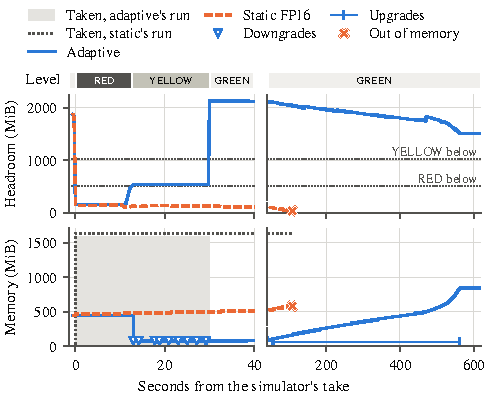
\includegraphics[width=\columnwidth]{figures/survival.pdf}
\caption{The adaptive engine under S6, S5's take released after 30\,s, and the
static FP16 engine under S5, its take kept, to where it ran out of memory; one run
each. Above, the level the adaptive run's monitor reported, the headroom and the
thresholds; below, each engine's cache and what its simulator took. Triangles are
the steps that found pages downgraded by a plan, and the bar spans the upgrades.
The time axis changes scale at 40\,s and ends at 620\,s; the adaptive run
completed its 32{,}767 positions at 4231\,s. The runs differ in commit and in
prompt, 30{,}720 positions and 2{,}048 decoded against 32{,}704 and 64.}
\label{fig:survival}
\end{figure}

\paragraph{Reacting during prefill.} Detection took 165\,ms, but with
512-position chunks every event during prefill waited for the chunk in
progress, 13.2\,s at the median. Table~\ref{tab:prefill} compares three runs.
A first design sized chunks under pressure from the time per position alone
and chose one 16-position tile at every step from 26K positions, each still
taking about 1.7\,s: a step has a large fixed part. Modelling that part brings
the median for events after an episode's first to 0.86\,s. The first event of
an episode still waits for the chunk in progress, and at 32K positions prefill
under pressure takes about 2.4 times as long, the price of acting within a
second or two.

\paragraph{Across scenarios.} The survival matrix runs the same generation under
static FP16, INT4 and INT2 engines and the adaptive engine from each score
source, in four scenarios that begin at 16{,}384 positions: a grid of pulses up
to 1408\,MiB (S1), a train of RQ1's P90 pulse (S2) and RQ1's spikes drawn at
its rate (S3), each on a base that leaves 1536\,MiB, and its desktop
recordings replayed from their own headroom (S4), three runs a cell
(Table~\ref{tab:matrix}). Only a static FP16 engine failed S1, in all three
runs. The static INT4 and INT2 engines survive by holding a quarter or an
eighth of the bytes from the first token; the adaptive ones by returning
372--642\,MiB when the pulses came and restoring FP16 after them. A static
INT8 engine completed every run, but on a later, faster build of the engine,
which finished the positions after contention in about 150\,s where the other
static engines took 600--760\,s; it met less of each schedule, at most 998\,MiB of S3's first
draw against 2205, so its row does not compare with the others'. S3's first
draw accumulated more than the device holds, and only the uniform source
completed it. An adaptive engine runs longer under pressure and so meets more
of a schedule, up to 1296\,s of S3 against the static engines' 665\,s. Three
runs cannot tell the sources apart, and the monitor missed no detectable RED
episode and raised no false one in any run. Events during prefill still waited
for the chunk in progress, 4.5--15.8\,s at the median by scenario: chunks are
sized by time only while pressure holds, and S1's and S2's pulses pass within
one.

\begin{table}[t]
\caption{Runs that completed every token, of three a cell in the pulse grid
(S1), the pulse train (S2), RQ1's arrivals (S3) and RQ1's replays (S4), or of
the survival experiment's one (S5, and S6, its release, which a static engine
has no upgrade path to exercise). llama.cpp, by its cache's type, ran S1 and S5
only, three runs each. A Wilson 95\% interval at 3/3 is
[44, 100]\%, at 2/3 [21, 94]\%. $^\dagger$Run on a faster build, and so
against less of each schedule.}
\label{tab:matrix}
\centering
\small
\begin{adjustbox}{max width=\columnwidth}
\begin{tabular}{lrrrrrr}
\toprule
& S1 & S2 & S3 & S4 & S5 & S6 \\
\midrule
Static FP16 & 0/3 & 3/3 & 1/3 & 3/3 & 0/1 & -- \\
Static INT4 & 3/3 & 3/3 & 2/3 & 3/3 & 1/1 & -- \\
Static INT2 & 3/3 & 3/3 & 2/3 & 3/3 & 1/1 & -- \\
Static INT8$^\dagger$ & 3/3 & 3/3 & 3/3 & 3/3 & 1/1 & -- \\
Adaptive, uniform & 3/3 & 3/3 & 3/3 & 3/3 & 1/1 & 1/1 \\
Adaptive, random & 3/3 & 3/3 & 2/3 & 3/3 & 1/1 & 1/1 \\
Adaptive, semantic & 3/3 & 3/3 & 2/3 & 3/3 & 1/1 & 1/1 \\
\midrule
llama.cpp, f16 & 3/3 & -- & -- & -- & 3/3 & -- \\
llama.cpp, q8\_0 & 3/3 & -- & -- & -- & 3/3 & -- \\
llama.cpp, q4\_0 & 3/3 & -- & -- & -- & 3/3 & -- \\
\bottomrule
\end{tabular}
\end{adjustbox}
\end{table}

\paragraph{A deployed engine.} llama.cpp ran the same model and generation, its
weights at FP16 and its cache at f16, q8\_0 and q4\_0, against the same bytes of
S1 and S5 (Appendix~\ref{app:llamacpp}). All 18 runs completed. It allocates the
whole cache as it loads, 896\,MiB at f16, so contention that comes later has
nothing left to refuse it; what it holds is refused to the process that asks. At
f16 the simulator was refused 340--364\,MiB at the worst of S1's pulses and some
part of them for 60 of its 494\,s, and 302--310\,MiB of S5's step. At q8\_0 and
q4\_0 it was refused nothing but 8\,MiB once, and the cache is at 8 or 4 bits
from the first token, as a static engine's is. In S1 the adaptive engine refused
nothing from the uniform source, and nothing in two runs of the semantic one's
three and 130\,MiB in the third; the static FP16 engine refused 244--274\,MiB
before it ran out. The out-of-memory failure is thus that of a cache
allocated as it grows. Reserving it averts the failure and moves the shortfall
to the other process; a narrower cache averts both here and is paid for throughout.
The adaptive engine holds FP16 until pressure comes and gives the memory up
then.

\subsection{RQ3: Quality at Equal Compression}
\label{sec:rq3}

RQ3 compares the semantic, uniform and random score sources, and ZipCache's
normalised attention \citep{he2024zipcache}, at equal reclaimed bytes. Compression is imposed by a \textit{controlled plan} between two turns of
a conversation: the engine is given a byte target, 70\% or 80\% of the FP16
bytes outside the recency floor, and a score source, and the same planner meets
it with no monitor involved, so that every source reclaims the same bytes and
runs repeat exactly. In the primary, question-blind experiment, turn~1 asks for
a summary of an 8K-position document, the plan is applied, and turn~2 asks for a
code planted at one of ten depths; whether attention paid before the question
predicts what is consulted after it is the premise under test. ZipCache's
score is each page's attention from probe tokens, a tenth of the positions,
divided by the probes that could attend to it. We take it by a pass over the
tokens already cached, before the question, so the same planner and bytes apply
(Appendix~\ref{app:zipcache}); the closing tests stay semantic against uniform. A
question-aware experiment, compressing after the question, bounds what a
query-aware allocation could do. Fifty samples, screened at FP16, are compared
by McNemar's exact test. Static INT4 and INT2 stand for uniform quantisation,
and eviction of the pages the semantic plan would degrade most, at the same
bytes, for H2O's family: attention over a cache with pages evicted equals, to
the bit, attention with them masked. Continuation fidelity teacher-forces 128
tokens of 50 WikiText-2 passages after a 2K-token prefix, and the anchor-fact
dialogue asks, after ten turns, for a code stated in one of them. Five of
RULER's tasks \citep{hsieh2024ruler} run the same two turns at 8K and 32K
positions: a key among four in essays (MK-1), one among needle-shaped fillers
of numbers (MK-2) or UUIDs (MK-3), four values of one key (MV), and variable
tracking along a chain of assignments (VT). Static INT2 answered at most 21 of
a task's 50 screened samples, so every task is below its ceiling of 40, and the
closing test, fixed before the runs, pools the five at each length.

\begin{table}[t]
\caption{RQ3 at 80\% of the bytes reclaimed, question-blind, on Qwen2.5-1.5B.
Needles and facts are of 50, continuation fidelity is top-1 agreement (\%) and
mean KL from FP16 over 50 passages. Effective bits are the needle set's; on
each task every adaptive condition held the same bits, and no needle-set plan
fell short. A static condition holds the whole cache at its tier. The four score
sources' rows were run beside each other at one commit, the others earlier.}
\label{tab:rq3}
\centering
\small
\begin{adjustbox}{max width=\columnwidth}
\begin{tabular}{lrrrrr}
\toprule
Condition & Bits & Needles & Facts & Top-1 & KL \\
\midrule
FP16 & 16.00 & 50 & 50 & 100 & 0 \\
Static INT8 & 8.63 & 50 & 50 & 99.7 & $<$0.001 \\
Static INT4 & 4.63 & 50 & 50 & 96.6 & 0.006 \\
Static INT2 & 2.63 & 45 & -- & -- & -- \\
Uniform & 3.40 & 49 & 44 & 86.5 & 0.101 \\
Random & 3.40 & 50 & 48 & 87.6 & 0.082 \\
Semantic & 3.40 & 48 & 48 & 93.7 & 0.028 \\
ZipCache & 3.40 & 48 & 49 & 92.8 & 0.036 \\
Eviction & 3.40 & 16 & 16 & -- & -- \\
\bottomrule
\end{tabular}
\end{adjustbox}
\end{table}

\textbf{On the needle set the closing comparison is null.} At 80\%, question-blind, the semantic
source answered 48 needles and uniform 49 (Table~\ref{tab:rq3}); one sample was
answered by uniform alone and none by semantic alone, McNemar's $p = 1$. It
stays null at 70\%, where every source answered all 50; with the question
seen, 49 against 50; on a 32K subset of ten, all 10 for both; and in an
end-to-end run, where the simulator's contention rather than a controlled
plan forced the reclamation, 48 against 49 on the same contention. The needle
set sits at its ceiling: static INT2 for the whole cache kept 45 of 50. The
semantic order did work as designed, leaving 43\% of the needles' pages at INT2
against uniform's 68\%, but the code survived INT2 in most samples whichever
source sent it there.

\begin{table}[t]
\caption{RULER, question-blind, on Qwen2.5-1.5B: samples answered of 50 at
70\% / 80\% of the bytes reclaimed, every string of the answer found. Bits are
4.98 / 3.40 at 8K and 4.84 / 3.25 at 32K for every source. The closing test
pools the five tasks at 80\%. ZipCache's score was run at 8K only.}
\label{tab:ruler}
\centering
\small
\begin{adjustbox}{max width=\columnwidth}
\begin{tabular}{llrrrrr}
\toprule
 & Task & INT2 & Semantic & Uniform & Random & ZipCache \\
\midrule
8K & MK-1 & 21 & 49 / 38 & 50 / 37 & 50 / 38 & 50 / 40 \\
 & MK-2 & 5 & 50 / 15 & 50 / 19 & 49 / 20 & 50 / 26 \\
 & MK-3 & 0 & 17 / 1 & 46 / 1 & 44 / 4 & 48 / 3 \\
 & MV & 2 & 41 / 20 & 31 / 13 & 34 / 9 & 47 / 15 \\
 & VT & 1 & 49 / 49 & 50 / 30 & 45 / 29 & 50 / 48 \\
 & All & 29 & 206 / 123 & 227 / 100 & 222 / 100 & 245 / 132 \\
\midrule
32K & MK-1 & 10 & 49 / 35 & 50 / 29 & 50 / 30 & -- \\
 & MK-2 & 0 & 35 / 6 & 46 / 3 & 43 / 4 & -- \\
 & MK-3 & 0 & 0 / 0 & 38 / 0 & 21 / 0 & -- \\
 & MV & 0 & 30 / 13 & 35 / 7 & 33 / 9 & -- \\
 & VT & 0 & 48 / 46 & 48 / 13 & 47 / 15 & -- \\
 & All & 10 & 162 / 100 & 217 / 52 & 194 / 58 & -- \\
\bottomrule
\end{tabular}
\end{adjustbox}
\end{table}

\textbf{Below its ceiling, semantic allocation answers more.} On RULER at
80\%, the semantic source answered 123 of 250 samples at 8K against uniform's
100, 40 samples by semantic alone and 17 by uniform alone ($p = 0.0032$), and
100 against 52 at 32K, 58 to 10 ($p = 2.4 \times 10^{-9}$): the closing test is
a yes at both lengths (Table~\ref{tab:ruler}). Variable tracking carries most
of it, 19 to 0 and 33 to 0; over the other four tasks the count is 21 to 17 at
8K and 25 to 10 at 32K. Where the plans left the answer shows why. On VT the
semantic source held 3\% of the answer's (layer, page) cells at INT2, against
uniform's 70\%; on MK-1 and MV 49--63\% against 66--74\%; on MK-2 and MK-3,
whose fillers question-blind attention cannot tell from the needle, 63--75\%
against 69--74\%.

\textbf{At 70\%, concentration costs.} Uniform allocation meets the 70\% target
without INT2; the semantic source spends the same bytes unevenly,
holding up to 13\% of the cache at INT2. Where it does not find the needle,
the INT2 lands on it: on MK-3 in 44 and 47 of 50 runs, and semantic answered
17 against uniform's 46 at 8K and 0 against 38 at 32K ($p < 10^{-7}$); on MK-2
at 32K, 35 against 46 ($p = 0.0034$). It won MV at 8K, 41 against 31. Over the
five tasks it answered 206 against 227 at 8K, 12 samples by semantic alone and 33
by uniform alone ($p = 0.0025$), and 162 against 217 at 32K, 6 to 61 ($p = 1.5
\times 10^{-12}$).

\textbf{A better score for 70\%.} That loss is the score's, not the planner's.
At 8K and 70\% ZipCache's source answered 245 of 250, 40 samples by it alone and 1
by semantic alone ($p = 4 \times 10^{-11}$), and 18 to 0 against uniform
($p = 8 \times 10^{-6}$): its scores sent at most 0.2\% of a task's cache to
INT2, against semantic's 1--9\%, and one MK-3 run in 50 had an INT2 cell on the
needle, against 44. At 80\% it answered 132 against semantic's 123, 24 to 15
($p = 0.20$), and 45 to 13 against uniform. It gives up the continuation at 80\%:
KL 0.036 against 0.028, semantic lower on 48 of 50 passages (paired difference
$-0.0076$ [$-0.0097$, $-0.0057$]), though at 70\% it is lower, 0.0010 against
0.0023, mostly by one passage. Needles and facts do not part them, 48 and 49 against 48 and 48. Its
pass over the prompt took 43\,s at 8K here; the scorer's scores come with decoding.

\textbf{Graded measures part the sources.} In continuation fidelity at 80\%,
semantic allocation kept the next-token distribution 3.6 times closer to FP16
than uniform, a paired difference in mean KL of $-0.073$ [$-0.082$,
$-0.065$], lower on all 50 passages (Figure~\ref{fig:pages}, top), and top-1
agreement 7.2 points higher.
At 70\% its KL against uniform's was within the interval, at 0.0023 against
0.0031. A whole cache at INT4, at 4.63 bits, between the two levels' 5.48 and
3.98, kept a KL of 0.0055, between semantic's at them; at INT8 it was
$2 \times 10^{-5}$. In the dialogue, semantic recalled 48 facts against uniform's 44, four
dialogues answered by semantic alone and none the other way ($p = 0.125$);
uniform held every fact's page at INT2, semantic 38\% of them.

\textbf{A second family.} On Llama-3.2-1B (Appendix~\ref{app:llama}), semantic
allocation answered 134 of 250 RULER samples at 8K and 80\% against uniform's 58,
80 samples by semantic alone and 4 by uniform alone ($p = 2 \times 10^{-19}$),
more on every task but MK-3, which neither answered, and without variable
tracking 52 to 3. Its needle set is below its ceiling (static INT2 26 of 50):
semantic 50, uniform 41 ($p = 0.0039$), though random's 46 is not told apart. The
KL from FP16 in continuation at 80\% was 0.050 against 0.194. The loss at 70\% on
MK-3 did not recur, 32 each. The adaptive engine survived S5, which ended the
static one, one run each.

\textbf{Downgrading keeps what eviction loses.} At the same bytes, eviction
answered 16 needles and recalled 16 facts at 80\%, and 22 and 21 at 70\%,
against semantic's 48, 48, 50 and 50; every sample eviction answered, semantic
did too ($p < 10^{-8}$ throughout). On RULER it answered most of
variable tracking, whose pages the plan held high; on Llama-3.2-1B there it was
not told apart from semantic (37 against 30 at 80\%, $p = 0.17$). In the dialogue at 80\% eviction kept the
facts of the last two turns and lost most stated three or more turns back.

\textbf{Recovery and ablations.} After pressure passes, restoring every page
from its shadow took under 0.7\,s at 8K positions; a third turn then answered
50 of 50 needles under semantic, both of its turn-2 misses recovered. At 32K,
a 30\,s pulse during prefill was survived by all three sources with every page
restored, about nine minutes after the release, the first seven of them prefill.
None of nine quality ablations at 80\% changed needle accuracy detectably
($p \ge 0.5$); planning by importance alone, without the tier's error, lost
the most, two samples. Two were not at equal bytes: without INT2, and with a
512-position recency floor, every plan fell short of its target.

\textbf{Does a page's score predict its damage?} At each task's plan point
we drew 64 pages a sample among those a plan may move, moved each alone to
INT4 on a conversation started from the plan point's snapshot, and
teacher-forced the measured tokens: the question and FP16's answer for the
needle and the dialogue, the 128 tokens for continuation. A page's damage is
the mean KL from FP16 over them; with no page moved the logits are FP16's to the
bit. Over 3{,}200 pages a task, Spearman's $\rho$ between score and damage was
$0.356$ [$0.307$, $0.401$] for continuation, positive in 49 passages of 50, but
$0.031$ [$-0.008$, $0.069$] on the needles and $0.068$ [$0.041$, $0.094$] in the
dialogue (95\% bootstrap over samples; Figure~\ref{fig:pages}, bottom); for ZipCache's
scores of the same pages,
$0.306$, $0.027$ and $0.050$. The score ranks pages by the damage
their downgrade does to the continuation of the text it watched, not by the
damage to the answer of a question asked after it, which agrees with the null
comparison on the needle set.

\begin{figure}[t]
\centering
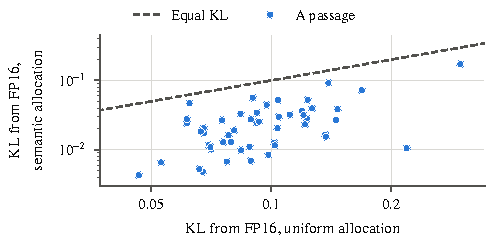
\includegraphics[width=\columnwidth]{figures/continuation.pdf}
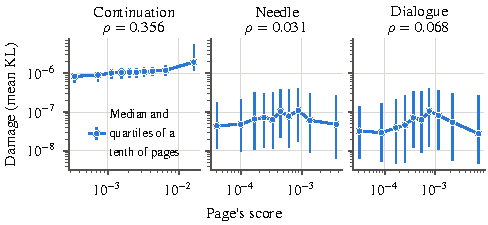
\includegraphics[width=\columnwidth]{figures/damage.pdf}
\caption{Top: each passage's mean KL from FP16 in continuation at 80\% of the bytes
reclaimed, semantic allocation against uniform's: every passage lies below the
line of equal KL. Bottom: a page's damage, the mean KL with it alone at INT4, against
its score on each task: the median and quartiles of each tenth of 3{,}200 pages
by score, with Spearman's $\rho$ over the pages. On
continuation it rises with the score; on the needle and in the dialogue it rises
to the middle of the scores and falls back.}
\label{fig:pages}
\end{figure}

\textbf{Answer.} At equal bytes, attention-guided allocation kept the model's
output distribution markedly closer to full precision than uniform allocation,
as a page's score predicts its damage there. It answered no more of a needle
set too easy to separate the sources; on RULER's tasks below their ceiling it
answered more at 80\% at both lengths, chiefly where the answer stands apart
from its context, and fewer at 70\% where needle-shaped fillers hide it, a loss
ZipCache's score, at the cost of a pass over the prompt, did not have. Which score
orders the pages is a choice the mechanism leaves open. At 80\% reversible
degradation kept three times the answers of eviction.

% =====================================================================
\section{Limitations}
\label{sec:limitations}

\textbf{One machine, and a second family on a subset.} Every measurement is from
one laptop GPU; the thresholds are set by a rule, so another machine changes their
values but not the method. Llama-3.2-1B, with eight key-value heads, ran continuation
fidelity, the needle set, RULER at 8K and S5 once; the survival matrix, the
correlation and the 32K results are of Qwen2.5 with two.
\textbf{Simulated contention.} RQ2 uses a simulator that takes memory but no
compute, isolating the variable studied; replays reproduce their originals to
within tens of MiB. \textbf{Rate.} RQ1 characterises the size and speed of
contention, not how often it occurs over a working day. \textbf{Few runs.}
Survival is three runs a cell in four scenarios and one in the step and the
release, which bound a rate only loosely and cannot tell the score sources
apart; an adaptive engine also meets more of a schedule than a static one.
\textbf{An external engine in part.} llama.cpp ran two scenarios, loaded before
contention came; its loading under contention and its quality at q8\_0 and q4\_0
are not measured. \textbf{Reacting at step boundaries.} The first event of an
episode waits for the step in progress, and at long contexts a step's fixed part exceeds a
second, so no chunk size meets a 1\,s target there. \textbf{Attention as a
signal.} We use attention mass as a predictor of which pages will be consulted
again, not as an explanation of the model; RQ3 tests that use by its outcome
and page by page, one page moved to INT4 at a time, which shows the ranking a
plan relies on but not how many pages' damages combine, nor the correlation at
INT2 or at 32K positions. \textbf{A task at its ceiling.} At 8K positions on
Qwen2.5-1.5B our needle's code survives INT2 in most samples, so at most five
samples could be discordant at 80\%, fewer than McNemar's test needs; RULER's
tasks, below their ceiling, are what separate the sources. \textbf{Where the
score cannot see the answer.} Question-blind attention does not single out a
needle among needle-shaped fillers, and there the semantic source's uneven
allocation put INT2 on the needle that uniform allocation spared at 70\%;
RULER's yes at 8K rests on variable tracking alone on Qwen2.5-1.5B, and only the
question-blind experiment was run on it. ZipCache's score was run question-blind
at 8K on Qwen2.5-1.5B only, through a pass of its own into a second FP16 cache,
so its cost at runtime, or under pressure, is not measured.

% =====================================================================
\section{Conclusion}
\label{sec:conclusion}

On a shared consumer GPU, memory an inference engine counts on changes for
reasons it neither causes nor sees. We showed that this contention is large,
rises over seconds and mostly persists; that a monitor consulting no scheduler
detects it within a quarter of a second; and that an engine which reallocates
cache precision at runtime, page by page, and returns the memory to the driver,
survives a contention that ends a static engine whose cache grows, in every run
of four scenarios that ended one but a draw that exceeded the device, where an
engine that reserves its cache survives by refusing that memory to others. At equal
bytes, allocating
that precision by attention kept the model's output closer to full precision
than allocating it uniformly, and more of RULER's answers at 80\% though fewer
at 70\% where our score could not find the needle and ZipCache's, on the same
planner, did not lose it; degrading pages reversibly kept far more than evicting
them.

% =====================================================================
% Unnumbered statements, outside the page limit, before the references.

\ificmlshowauthors
\section*{Acknowledgements}

The author thanks Ng\^o V\u{a}n Linh for supervising this work, and for
insisting that a systems claim is only as good as the measurement behind it.
\fi

\section*{AI Use Statement}

% TODO(owner): confirm that this statement matches how AI tools were used, as
% ICML 2027's policy on generative AI requires.
An AI coding assistant, Claude Code, was used throughout this work: to write
and test parts of the engine's code under the authors' design and review, to
prepare and run experiments to protocols the authors fixed beforehand, and to
draft and revise the text of this paper. Every claim was checked by the authors
against the benchmark log, from which every figure quoted is drawn, and the
authors take full responsibility for the content of the paper. No AI tool is
part of the method studied; the language models evaluated are its subject.

\section*{Impact Statement}

This paper presents work whose goal is to make language model inference on
personal hardware more reliable. Local inference keeps user data on the user's
machine and needs no datacenter; we see no negative impact particular to this
work beyond those of the language models it serves.

\bibliography{references}
\bibliographystyle{icml2027}

% =====================================================================
% APPENDIX
% =====================================================================
\newpage
\appendix
\onecolumn

\section{Analysing Contention Traces}
\label{app:spikes}

Free memory is sampled at 50\,Hz. Its baseline is the rolling median of the
preceding 5\,s, and a spike is free memory at least 64\,MiB below the baseline
for at least 100\,ms. Four rules make the definition hold on a real trace.
\begin{itemize}
\item The baseline holds during a spike, for one window at most; a spike still
below it after a window is a \textit{lasting drop}, and the new level becomes
the baseline.
\item A spike ends only when its deficit falls below half the threshold, so
noise does not split it.
\item A gap in the trace ends a spike, which is then censored.
\item A measure stays within its own spike.
\end{itemize}
The amplitude is the largest deficit; the rise time runs from 10\% of the
amplitude to the start of its 90\% peak; the duration is the time at or above
the threshold. A spike is attributed to the process whose memory gained most
between the last 5\,Hz sample before the rise and the samples during the peak,
if it gained at least a quarter of the amplitude.

\begin{figure}[!ht]
\centering
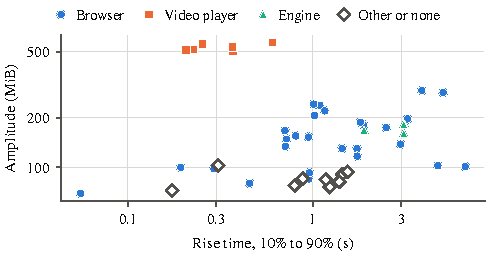
\includegraphics[width=\columnwidth]{figures/spikes.pdf}
\caption{RQ1's spikes: amplitude against rise time, by the process each is
attributed to. The video player takes the most, in 0.2 to 0.6\,s; the browser's
spikes are smaller, and 16 of its 27 rise over a second or more. One of the 48, with no
rise measured, is not shown.}
\label{fig:spikes}
\end{figure}

\section{The Contention Simulator}
\label{app:simulator}

The simulator is a process with its own CUDA context, so its memory is another
process's to the driver. It launches no kernel and takes memory through the
engine's VMM allocator, a granule at a time, following a schedule of bytes over
time with absolute deadlines. A change of 64\,MiB is visible to the driver
13\,ms after it is due, and one of 1\,GiB after 208\,ms. Schedules are
synthetic trapezoids of a given amplitude, ramp and plateau, or replays of what
the processes other than the engine held in an RQ1 recording, played on a base
that leaves the original's headroom.

\section{The Survival Experiment}
\label{app:survival}

Table~\ref{tab:survival} gives the two runs of the survival experiment, and
Table~\ref{tab:prefill} the time from a pressure event during prefill to its plan
under three rules for sizing chunks (Section~\ref{sec:survival}).

\begin{table}[!ht]
\caption{The survival experiment at 32K positions. The static engine runs out
of memory; the adaptive one (semantic) completes, and the driver sees every
byte it returns.}
\label{tab:survival}
\centering
\small
\begin{adjustbox}{max width=\columnwidth}
\begin{tabular}{lrr}
\toprule
& Static FP16 & Adaptive \\
\midrule
Ending & OOM at 20{,}992 & complete, 32{,}767 \\
Headroom at the take / taken (MiB) & 1904 / 1630 & 1883 / 1610 \\
Lowest free after the take (MiB) & 11 & 159 \\
Plans / downgrades & 0 / 0 & 33 / 85{,}596 \\
Returned / seen by the driver (MiB) & -- & 746 / 746 \\
Plans matching the driver to a granule & -- & 32 of 32 \\
\bottomrule
\end{tabular}
\end{adjustbox}
\end{table}

\begin{table}[!ht]
\caption{From a pressure event during prefill to its plan, at 32K positions,
with chunks of 512 positions, chunks sized by the time per position, and chunks
sized by a fixed and a per-position part. Modelling the fixed part brings
later events within about a second; the first event of an episode still waits
for the chunk in progress.}
\label{tab:prefill}
\centering
\small
\begin{adjustbox}{max width=\columnwidth}
\begin{tabular}{lrrr}
\toprule
& 512 & Per position & Fixed + per position \\
\midrule
First event of the episode & 11.1\,s & 11.1\,s & 11.1\,s \\
Later events, median & 13.2\,s & 1.5\,s & 0.86\,s \\
Later events within 1\,s & 0 & 24 of 74 & 3 of 5 \\
From the take to the end & 668\,s & 1617\,s & 1588\,s \\
\bottomrule
\end{tabular}
\end{adjustbox}
\end{table}

\section{The From-Scratch Boundary}
\label{app:boundary}

Every kernel the contribution touches is hand-written CUDA; the dense
projections call \texttt{cublasGemmEx} through one wrapper, with fp16 operands,
fp32 computation and reduced-precision reduction disallowed, and a projection's
bias seeded into its output so that the result is rounded once. A naive GEMM
and a shared-memory-tiled one, profiled against cuBLAS with Nsight Compute,
ran 93--267 and 8--28 times slower at 512 rows, the naive kernel bound by its
load and store queue, the tiled one by shared memory, and cuBLAS by tensor
cores; they are a study, tested to stay off the inference path.

\section{A Second Model Family: Llama-3.2-1B}
\label{app:llama}

Llama-3.2-1B-Instruct has 16 layers, eight key-value heads of 64 dimensions, no
projection bias and scaled rotary frequencies; 32K positions take 1\,GiB at FP16.
Its sealed pages cost 8.75, 4.75 and 2.75 effective bits at INT8, INT4 and INT2,
and plans are held to equal bytes as on Qwen2.5-1.5B. Against a float32
HuggingFace reference, the engine's greedy token at FP16 agrees at 99.98\% of
5{,}689 positions and its mean KL is $9.8 \times 10^{-7}$; each narrower tier
costs more (on the 8-prompt tier subset, mean KL $5.3 \times 10^{-6}$ at INT8,
$1.2 \times 10^{-3}$ at INT4, $7.4 \times 10^{-2}$ at INT2). The samples are
screened for this model, so they are not Qwen2.5-1.5B's.

\begin{table}[!ht]
\caption{RULER at 8K on Llama-3.2-1B, question-blind: samples answered of 50 at
70\% / 80\% of the bytes reclaimed. Bits are 4.98 / 3.40 for every source. Static
INT2 leaves every task below its ceiling of 40; the closing test pools the five
at 80\%.}
\label{tab:llama}
\centering
\small
\begin{tabular}{lrrrrrrr}
\toprule
Task & INT2 & INT4 & INT8 & Semantic & Uniform & Random & Eviction \\
\midrule
MK-1 & 20 & 50 & 50 & 50 / 43 & 50 / 29 & 49 / 34 & 24 / 22 \\
MK-2 & 6 & 46 & 50 & 47 / 25 & 48 / 15 & 48 / 22 & 6 / 4 \\
MK-3 & 0 & 31 & 49 & 32 / 0 & 32 / 0 & 27 / 0 & 1 / 1 \\
MV & 1 & 41 & 49 & 45 / 36 & 45 / 11 & 41 / 8 & 11 / 4 \\
VT & 0 & 24 & 41 & 42 / 30 & 31 / 3 & 33 / 3 & 39 / 37 \\
All, 80\% & & & & 134 & 58 & 67 & 68 \\
\bottomrule
\end{tabular}
\end{table}

\paragraph{RULER.} At 80\% the answered share differs by $+0.304$ [$0.244$, $0.364$].
The answered samples were 15 to 1 on MK-1, 11 to 1 on MK-2, 26 to 1 on MV and 28 to 1
on VT (each $p \le 0.0064$), and the pooled count against random 73 to 6. Where the
plans left the answer parts the sources on three tasks: semantic held 50\% of MK-1's (layer, page)
cells at INT2 against uniform's 84\%, 41\% of MV's against 71\% and 12\% of VT's
against 76\%; on MK-2, however, both held 76\%, so its gain there is not the
needle's tier. At 70\% semantic answered 216, uniform 206 and random 198, 20 to 10
against uniform ($p = 0.099$). FP16 answered 50 of 52, 56, 120, 95 and 177 drawn
(MK-1, MK-2, MK-3, MV, VT), so VT's and MK-3's screened sets hold 28\% and 42\% of
their draws. RULER allows 30 tokens for VT's answer: 57 of the 127 VT samples FP16
missed ran to that limit, and so did 18 of the 50 it answered.

\paragraph{Continuation and needles.} At 80\% the mean KL was 0.050 for semantic,
0.194 for uniform and 0.158 for random, lower than each on all 50 passages
(paired difference from uniform $-0.144$ [$-0.159$, $-0.130$]), and top-1 agreement
89.7, 80.1 and 81.5\%; at 70\%, 0.0017, 0.0049 and 0.0089. On the needle set
semantic answered 50, uniform 41 and random 46 at 80\%, 9 samples by semantic alone
against uniform and 4 against random, none the other way ($p = 0.0039$, $0.125$);
all 50 at 70\%.

\paragraph{Survival.} In S5, the static engine ran out of memory at 23{,}040
positions and the adaptive engine completed all 32{,}767 in 154 plans, returning
910\,MiB that the driver saw, every plan to a granule. One run each.

\clearpage % keep the heading and both tables of this section on one page
\section{ZipCache's Score as a Source}
\label{app:zipcache}

ZipCache ranks a token by its normalised attention, the attention it receives
divided by the queries that could attend to it, read from probe tokens, the most
recent 5\% of positions and a random 5\%. We run that rule as a score source of
the same planner, with three differences. Its probes are a step of one position
each in a second FP16 cache fed the conversation's tokens, so the cache a plan is
made on is the same, to the bit, for every source; in ZipCache the probes are in
its one prefill, so the pass's 43\,s at 8K positions is the experiment's and not
the method's. A layer's masses average its heads, and each layer's pages are
scored by their own layer. And the planner, not a saliency ratio between two
bit-widths, spends the bytes. Every one of the 1{,}700 plans met its target, by
less than 8\,KB. On the needle set, the dialogue and continuation the other
sources were run again at the same code. On RULER they are the runs of an earlier
commit, of which a check of 16 runs at the later code reproduced every one. Per
task at 8K and 70\%, ZipCache's source against uniform: 16 to 0 on MV
($p = 3 \times 10^{-5}$), 2 to 0 on MK-3, no other difference; at 80\%, 18 to 0
on VT, 9 to 2 on MK-2 ($p = 0.065$), 10 to 8 on MV, 5 to 2 on MK-1 and 3 to 1 on
MK-3. Against semantic at 80\%, 12 to 1 on MK-2 ($p = 0.0034$) is the only task
that parts them, and MV leans the other way, 4 to 9 ($p = 0.27$).

\section{llama.cpp Under the Same Contention}
\label{app:llamacpp}

llama.cpp's server (release b12300, commit ccd360f, built from source with CUDA)
ran Qwen2.5-1.5B converted at FP16 from the checkpoint MicroInfer runs: a 32K
context in one slot, every layer on the device, flash attention at every cache
type, as a quantised value cache needs, and batches of 512, MicroInfer's chunk.
Each run starts a server of its own, fills its cache to exactly 16{,}384 positions
by a completion of no tokens, and completes the 32{,}704-position prompt and 64
tokens once the simulator has taken its first level. S1's base and S5's shortfall
are set from the headroom an FP16 MicroInfer would have there, counting
llama.cpp's preallocated cache as one of the positions held, so that the bytes
taken are the same. One generation lasts 8--9\,s from the contention's
position and would meet a few of S1's pulses, so it is made again, the cache cut
back to 16{,}384 positions, until the schedule has been played: 57--64
generations a run, each of them complete in every run. Refused contention is the
most, over a run's levels, that the simulator asked for and was not given.
MicroInfer's comes from the events its matrix runs recorded; those runs, on the
build before split-key decode, met all of S1 where they completed. In S5 its
simulator was refused nothing by any engine, one run each: the step comes while the cache
has still half its growth to make. llama.cpp's S5 runs took 1176--1258\,MiB of
1486--1560 asked at f16 and all of 1480--1554 at q8\_0 and q4\_0. From the load to
the contention its memory grew by 16--28\,MiB. Its prefill ran at
2{,}338--2{,}620 positions a second, an order of magnitude faster than
MicroInfer's, and its decoding at 34--42 tokens a second; the runs were not made
to compare the two engines' speeds.

\section{The Cost of a Tier and of a Move}
\label{app:moves}

\begin{table}[!ht]
\caption{Each tier on Qwen2.5-1.5B: the footprint of a 32K cache, open pages
included, the effective bits of a sealed page with its metadata counted, and
WikiText-2 perplexity with the whole cache at the tier. INT2 is too lossy for a
whole cache, but not necessarily for the pages the model hardly attends to.}
\label{tab:tiers}
\centering
\small
\begin{tabular}{lrrr}
\toprule
Tier & 32K footprint (MiB) & Effective bits & Perplexity \\
\midrule
FP16 & 896 & 16.00 & 9.640 \\
INT8 & 486 & 8.63 & 9.641 \\
INT4 & 262 & 4.63 & 9.698 \\
INT2 & 150 & 2.63 & 11.541 \\
\bottomrule
\end{tabular}

\vspace{1.5em}
\caption{The time to move one page of one layer on Qwen2.5-1.5B, median of 256
moves. Copying the shadow on a first downgrade takes about 7\,$\mu$s of the
move. Below, decode throughput at 32K positions with the whole cache at each
tier, one run of 32 steps each, all at the same commit.}
\label{tab:moves}
\centering
\small
\begin{tabular}{lr}
\toprule
Move & Median ($\mu$s) \\
\midrule
FP16 to INT8 / INT4 / INT2 & 13 / 19 / 30 \\
The same, a first downgrade, copying the shadow & 23 / 29 / 39 \\
INT8 to INT4 / INT2, from the shadow & 32 / 37 \\
INT4 to INT8 / INT2, from the shadow & 21 / 37 \\
INT2 to INT8 / INT4, from the shadow & 21 / 26 \\
Any tier to FP16, from the shadow & 8 \\
\midrule
Decode at 32K, FP16 / INT8 / INT4 / INT2 (tokens/s) & 0.580 / 0.760 / 0.441 / 0.301 \\
\bottomrule
\end{tabular}
\end{table}

\end{document}
